\documentclass[varwidth=true, border=2pt]{standalone}
\usepackage{tikz}
\usepackage{tqft}

\begin{document}
    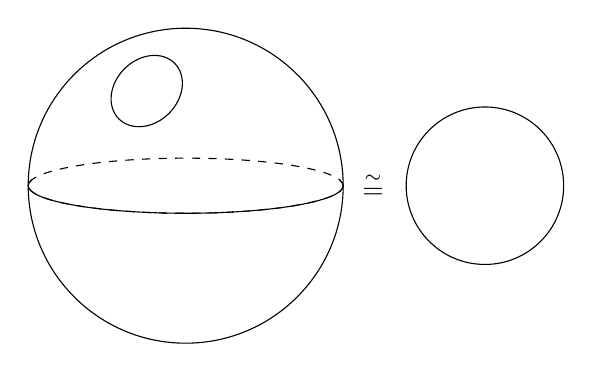
\begin{tikzpicture}[tqft/flow=east]
        \draw (0,0) circle (2cm);
        \draw (0,0) ellipse (2cm and 0.35cm);
        \draw[white,fill=white] (0,0.1) ellipse (1.95cm and 0.35cm);
        \draw[dashed] (0,0) ellipse (2cm and 0.35cm);

        \begin{scope}[rotate=45]
            \draw (0.5,1.2) ellipse (0.5cm and 0.4cm);
        \end{scope}

        \node at (2.38,0) {$\stackrel{\sim}{=}$};

        \draw (3.8,0) circle (1cm);
    \end{tikzpicture}
\end{document}
